%! Mode:: "TeX:UTF-8"
%! TEX program = xelatex
\documentclass[bwprint]{cumcmthesis}
\usepackage{ctex}
\usepackage{amsmath,amssymb,bm,booktabs,tabularx,array,longtable,enumitem}
\usepackage{graphicx}
\usepackage{float}
\usepackage{hyperref}
\usepackage[numbers,sort&compress]{natbib}
\usepackage{url}
\usepackage{subcaption}
\setCJKfamilyfont{kai}[AutoFakeBold]{FandolKai-Regular.otf}

\newcolumntype{C}{>{\centering\arraybackslash}X}
\newcolumntype{L}{>{\raggedright\arraybackslash}X}
\title{定日镜场的优化设计}
\tihao{A}
\baominghao{}
\schoolname{}
\membera{}
\memberb{}
\memberc{}
\supervisor{}
\yearinput{2023}
\monthinput{9}
\dayinput{10}
\makeatletter
\renewcommand*\mcm@commit@string@titlea{2023 高教社杯全国大学生数学建模竞赛}
\renewcommand*\mcm@numberpage@string@titlea{2023 高教社杯全国大学生数学建模竞赛}
\makeatother

\begin{document}
\pagenumbering{gobble}
\begin{abstract}
本文研究圆形区域内塔式太阳能光热电站定日镜场的光学性能评价与优化设计。全文将围绕统一的太阳位置、定日镜姿态、光学效率和热功率计算口径展开，并在该评价口径上依次处理给定镜场评价、统一规格镜场设计和逐镜可变规格镜场设计三个问题。

\textbf{针对问题一，}\pending{写入经审查的光学评价方法、给定1745面定日镜的年平均效率、年平均输出热功率与单位面积输出，并给出误差或敏感性证据。}

\textbf{针对问题二，}\pending{写入人类批准的统一规格优化方法、可行设计参数、60 MW约束裕量、单位面积输出及相对基线比较。}

\textbf{针对问题三，}\pending{写入人类批准的逐镜可变规格方法、最终设计、相对问题二的稳定增益与新增复杂度。}

\pending{摘要结论、物理含义和贡献表述只能从最终solution package、冻结数值及人类决策记录写入。}

\keywords{定日镜场\quad 光学效率\quad 太阳能光热\quad 约束优化}
\end{abstract}


\pagenumbering{arabic}
\section{问题重述}
题目计划在东经$98.5^\circ$、北纬$39.4^\circ$、海拔$3000$ m处建设半径为$350$ m的圆形定日镜场。镜场坐标系以建设区域中心为原点，$x$轴向东、$y$轴向北、$z$轴竖直向上。规划吸收塔高度为$80$ m，塔顶集热器为高$8$ m、直径$7$ m的圆柱形外表受光式集热器，吸收塔周围$100$ m内不得布置定日镜。

定日镜为宽度不小于高度的矩形，边长均须位于$2$--$8$ m，安装高度位于$2$--$6$ m，并保证镜面转动时不触地。相邻定日镜底座中心距离应比镜面宽度至少多$5$ m。题目规定年均指标使用每月21日$9{:}00$、$10{:}30$、$12{:}00$、$13{:}30$和$15{:}00$五个时点计算。

\textbf{问题一：}吸收塔位于区域中心，全部定日镜尺寸为$6$ m$\times6$ m、安装高度为$4$ m，镜心位置由附件给定。计算月平均和年平均光学效率、输出热功率及单位镜面面积输出热功率。

\textbf{问题二：}在全部定日镜尺寸及安装高度相同的条件下，设计吸收塔位置、镜面尺寸、安装高度、镜数和镜位，使年平均输出热功率达到$60$ MW，并使单位镜面面积年平均输出热功率尽量大。

\textbf{问题三：}允许各定日镜尺寸和安装高度不同，在相同额定功率条件下重新设计镜场，并继续提高单位镜面面积年平均输出热功率。

\section{总体分析}
三个问题共享同一条计算主线。问题一首先需要形成可复核的光学评价内核：由日期和时点确定太阳方向与法向直接辐射辐照度，再由太阳入射方向和镜心指向集热器中心的方向确定定日镜姿态，分别计算余弦、大气透射、阴影遮挡、截断和反射效率，最后汇总为镜场热功率与月、年指标。

问题二和问题三不应另行改变评价口径，而应把问题一的计算内核作为候选镜场的统一评价器。问题二的设计变量采用统一镜面尺寸与安装高度；问题三进一步放开逐镜尺寸和高度。两问均需同时处理场界、塔周禁布区、旋转离地、镜间距和$60$ MW额定功率约束。

因此，全文框架按“统一评价内核$\rightarrow$约束可行性$\rightarrow$候选设计比较$\rightarrow$高精度复算”的顺序组织。候选搜索阶段允许使用经记录和验证的近似，但最终表格、Excel提交文件和论文数值必须来自同一套冻结结果。

问题一采用经建模者确认的耦合低差异光线追迹作为正式数值求解器，并以低分辨率因子化光线追迹作为可完成全部输出的基线。主方法和基线共享同一连续光学模型，区别只在积分离散方式；后续问题应沿用问题一已经验证的太阳角、反射、阴影遮挡、有限圆柱截断和功率聚合口径。

\section{模型假设}
三个问题使用同一光学评价器，问题二和问题三只改变设计变量与约束，并不重新定义太阳辐射、反射和能量聚合方式。因此，下列假设同时适用于三问；坐标范围、给定镜场规模和集热器尺寸等题面事实不列作假设。

\begin{enumerate}[itemindent=2em]
  \item \textbf{全年晴空假设。}假设全年规定评价时段均为晴天，不考虑云层对太阳直射辐射的随机遮蔽，法向直接辐射强度统一由题目给定的DNI公式计算。该假设使各月规定时刻能够在相同气象口径下比较，但所得年平均功率不包含阴雨天气和云量变化造成的实际可利用率损失。
  \item \textbf{理想平面镜假设。}定日镜没有题面未给出的面形、斜率和跟踪误差，镜面法向使太阳中心光线指向集热器中心。该假设使反射几何可唯一确定，但真实电站的截断效率可能更低。
  \item \textbf{均匀太阳盘假设。}太阳锥采用半角$4.65\times10^{-3}$ rad、单位立体角能量均匀的pillbox分布。题面没有提供周日比，故不额外引入需要经验参数的周日区模型；问题一再用半角$\pm5\%$检验该简化对功率的影响。
  \item \textbf{联合光线计损假设。}阴影和遮挡均按每条光线的布尔可见性判断，多镜相交不重复计损；截断效率以未受阴影遮挡的反射光为条件分母。这是使题面效率乘积符合能量守恒的必要口径。
  \item \textbf{离散年平均假设。}每月五个规定时点等权形成月平均，十二个月等权形成题面离散年平均。三问均采用这一口径，使评价与优化目标一致；它不等同于逐日全年积分，问题一另与按月天数加权结果比较。
  \item \textbf{塔身与集热器几何。}三问均把塔身表示为半径3.5 m、$0\le z<72$ m的实体圆柱并计入入射阴影；集热器侧面取$72\le z\le80$ m，只在反射后的命中判定中使用。到达集热器侧面的反射能量按题面公式计入输出热功率，不额外加入未给出的吸收率或热损失。
\end{enumerate}

\section{符号说明}
\begin{table}[H]
\centering
\caption{三个问题共用的太阳与光学模型符号}
\begin{tabularx}{\textwidth}{>{\centering\arraybackslash}p{0.18\textwidth}L>{\centering\arraybackslash}p{0.14\textwidth}}
\toprule
符号 & 含义 & 单位 \\
\midrule
$\alpha_s$ & 太阳高度角 & rad \\
$\gamma_s$ & 太阳方位角 & rad \\
$\varphi$ & 当地纬度，北纬为正 & rad \\
$\omega$ & 太阳时角 & rad \\
$\delta$ & 太阳赤纬角 & rad \\
$D$ & 以春分为第0天起算的天数 & d \\
$\mathrm{DNI}$ & 法向直接辐射辐照度 & kW/m$^2$ \\
$N$ & 定日镜总数 & 面 \\
$A_i$ & 第$i$面定日镜采光面积 & m$^2$ \\
$\eta_i$ & 第$i$面定日镜光学效率 & -- \\
$E_{\mathrm{field}}$ & 定日镜场输出热功率 & kW \\
$\eta_{\mathrm{sb}}$ & 阴影遮挡效率 & -- \\
$\eta_{\cos}$ & 余弦效率 & -- \\
$\eta_{\mathrm{at}}$ & 大气透射率 & -- \\
$\eta_{\mathrm{trunc}}$ & 集热器截断效率 & -- \\
$\eta_{\mathrm{ref}}$ & 镜面反射率 & -- \\
$d_{\mathrm{HR}}$ & 镜面中心到集热器中心的距离 & m \\
$\boldsymbol{s},\boldsymbol{s}'$ & 太阳中心方向及太阳盘内方向单位向量 & -- \\
$\boldsymbol{t}_i,\boldsymbol{n}_i$ & 第$i$面镜指向接收器的方向及镜面单位法向 & -- \\
$\beta_i,\tau_i$ & 第$i$面镜法向方位角及镜面相对水平面的倾角 & rad \\
$\boldsymbol{e}_{w,i},\boldsymbol{e}_{h,i}$ & 第$i$面镜局部宽向、高向单位向量 & -- \\
$\theta_\odot$ & 均匀太阳盘半角 & rad \\
$J_i,T_i$ & 入射光相对其他镜面、塔身的可见指示量 & -- \\
$I_i,O_i,H_i$ & 联合入射可见、出射可见及集热器命中指示量 & -- \\
$\mathcal{C}_T$ & 半径3.5 m、高72 m的塔身实体圆柱 & m坐标集合 \\
$\mathcal{M}_i,\Omega_i$ & 有限矩形镜面及镜面点--太阳方向联合样本空间 & -- \\
$P_A$ & 单位镜面面积年平均输出热功率 & kW/m$^2$ \\
\bottomrule
\end{tabularx}
\end{table}

\begin{table}[H]
\centering
\caption{问题二与问题三的主要优化符号}
\begin{tabularx}{\textwidth}{>{\centering\arraybackslash}p{0.20\textwidth}L>{\centering\arraybackslash}p{0.14\textwidth}}
\toprule
符号 & 含义 & 单位 \\
\midrule
$k$ & 题目规定的太阳状态序号，$k=1,\ldots,60$ & -- \\
$\mathrm{DNI}_k,D_k$ & 第$k$个太阳状态的法向直接辐射辐照度 & kW/m$^2$ \\
$(x_T,y_T)$ & 吸收塔在建设场地内的平面坐标 & m \\
$(x_i,y_i,z_i)$ & 问题三第$i$面定日镜的镜心坐标 & m \\
$w,h,z_H$ & 问题二全场统一的镜宽、镜高和安装高度 & m \\
$w_i,h_i,a_i$ & 问题三第$i$面镜的宽度、高度及面积，$a_i=w_ih_i$ & m，m，m$^2$ \\
$A_{\mathrm{tot}}$ & 镜场总采光面积 & m$^2$ \\
$P_k,\overline P_{\mathrm{field}},\overline P$ & 状态输出功率及问题二、三的年平均输出热功率 & MW \\
$\mathcal D,\mathcal D_3$ & 问题二、三的完整设计变量集合 & -- \\
$d_{ij}$ & 第$i$、$j$面定日镜的镜心距离 & m \\
$R_b$ & 问题三内、外径向区域的分界半径 & m \\
$\phi_q$ & 区域$q$的三角点阵纵向平移相位，占一个点阵行距的比例 & 周期 \\
$d_q,\Delta y_q$ & 区域$q$的三角点阵最近邻间距与相邻行距 & m \\
$\rho_q$ & 区域$q$的基础镜面高宽比，$\rho_q=h_q/w_q$ & -- \\
$c$ & 镜面下缘相对地面的净空参数 & m \\
$\alpha$ & 问题三容量修复时两组逐镜规格之间的插值系数 & -- \\
\bottomrule
\end{tabularx}
\end{table}

\section{问题一：给定镜场的光学性能评价}

\subsection{问题分析与建模主线}

问题一并非只需把题面给出的五项效率代入乘积公式。余弦效率取决于每面镜的三维姿态，阴影与遮挡取决于光线在反射前后的有向路径，截断效率又取决于太阳并非单一平行方向以及接收器具有有限尺寸。因此，必须先定义从太阳辐射到圆柱接收器接收能量的连续物理映射，再选择数值方法求解其中的几何积分。

本问固定吸收塔平面坐标为$(0,0)$，按修订几何口径取集热器中心为$(0,0,76)$ m。附件给出1745面定日镜的镜心平面坐标；每面镜为$6\ \mathrm{m}\times6\ \mathrm{m}$，镜心高度均为4 m，总采光面积为$62820\ \mathrm{m^2}$。题目规定每月21日的9:00、10:30、12:00、13:30和15:00作为代表时点，故评价集合共有$12\times5=60$个状态。

图\ref{fig:q1-workflow}先给出本问的完整建模链。图中左栏回答“每一步计算什么”，右栏紧接着回答“为什么必须先做这一步”；左栏纵向箭头表示前一步是后一步的输入或定义基础，最下方虚线框才表示数值求解层。低差异采样、GPU分块和采样数只用于近似求解已经定义的连续积分，不参与定义太阳角、阴影、遮挡或截断效率。

\begin{figure}[H]
  \centering
  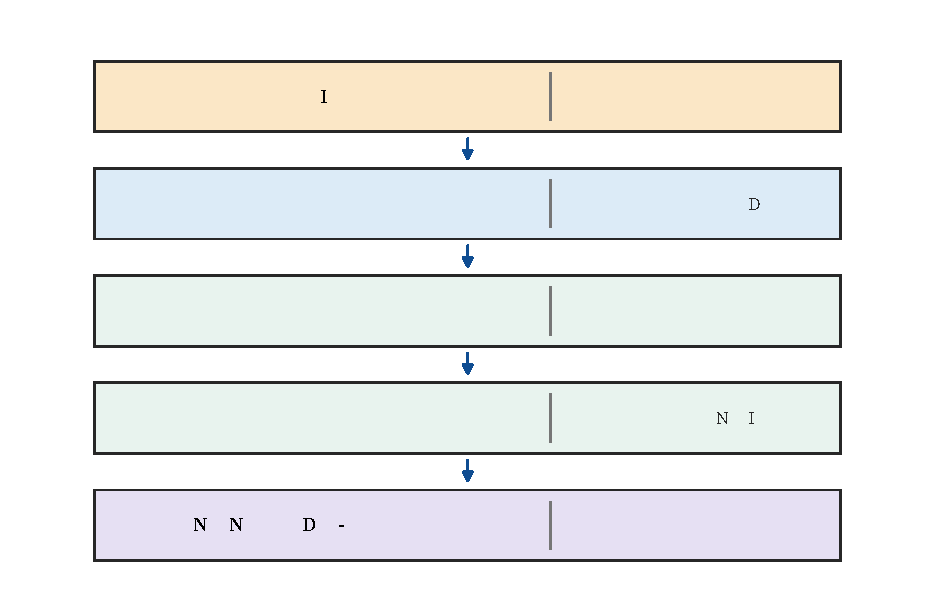
\includegraphics[width=0.98\textwidth]{figures/q1_model_workflow_cn.pdf}
  \caption{问题一各建模步骤、采用原因及数值求解边界}
  \label{fig:q1-workflow}
\end{figure}

由图\ref{fig:q1-workflow}可见，本问按“太阳输入$\rightarrow$镜面几何$\rightarrow$联合样本$\rightarrow$有向光路事件$\rightarrow$条件效率$\rightarrow$逐状态功率与聚合”的顺序建模。每一步都解决下一步的必要前提：太阳方向统一全部光学输入，有限镜面使相交事件可定义，联合样本保证各项损失针对同一份能量，条件截断保证效率乘积符合能量守恒，逐状态功率则保留DNI与效率的同步变化。因此，流程不是计算模块的简单罗列，而是一条不能任意交换顺序的物理推导链。

\subsection{坐标系、基本假设与适用范围}

建立右手直角坐标系：$x$轴向东，$y$轴向北，$z$轴竖直向上。太阳方位角从正北顺时针量取。按本文采用的几何口径，塔身是半径3.5 m、$0\le z<72$ m的实体圆柱；集热器侧面为半径3.5 m、$72\le z\le80$ m的有限圆柱侧面，中心为$(0,0,76)$。阴影表示入射光到达目标镜之前被其他镜面或塔身截断，遮挡表示反射光到达接收器区域之前被其他镜面截断；同一条光线即使与多个物体相交，也只记一次损失。

在题面没有给出额外参数的部分，采用以下经确认的简化：定日镜为理想平面镜，不加入面形误差、斜率误差和跟踪误差；太阳锥采用半角$\theta_\odot=4.65\times10^{-3}$ rad的均匀pillbox太阳盘；五个时点等权形成月平均，十二个月等权形成题面离散年平均；到达圆柱侧面的反射能量按题面公式全部计入输出热功率，不再擅自乘入接收器吸收率。

因此，后文“年平均”专指60个规定状态的等权离散平均，不是逐日逐小时气象积分；所得光学性能也只对应理想平面镜和均匀pillbox太阳盘，不直接等同于包含污染、跟踪误差和热损失的实际电站年发电量。

\subsection{步骤一：由规定时点确定太阳位置与DNI}

令状态集合为
\begin{equation}
\mathcal{T}=\left\{(m,h):m=1,\ldots,12;\ h\in\{9,10.5,12,13.5,15\}\right\}.
\end{equation}
对$t=(m,h)\in\mathcal{T}$，记每月21日相对春分的天数为$D_m$，当地纬度为$\varphi=39.4^\circ$。根据题面附录，赤纬角、时角与高度角依次满足
\begin{equation}
\sin\delta_m=\sin\left(\frac{2\pi D_m}{365}\right)\sin 23.45^\circ,
\qquad \omega_h=\frac{\pi}{12}(h-12),
\end{equation}
\begin{equation}
\sin\alpha_s(t)=\cos\delta_m\cos\varphi\cos\omega_h+
\sin\delta_m\sin\varphi.
\end{equation}

题面只给出方位角余弦，反余弦本身不能区分上午和下午。先计算
\begin{equation}
C_\gamma(t)=\frac{\sin\delta_m-\sin\alpha_s(t)\sin\varphi}
{\cos\alpha_s(t)\cos\varphi},
\end{equation}
再利用时角补足象限：
\begin{equation}
\gamma_s(t)=
\begin{cases}
\arccos C_\gamma(t), & \omega_h\le 0,\\
2\pi-\arccos C_\gamma(t), & \omega_h>0.
\end{cases}
\end{equation}
这样定义后，上午太阳位于东侧，下午位于西侧，正午位于南侧。镜场指向太阳中心的单位向量为
\begin{equation}
\boldsymbol{s}(t)=
\begin{bmatrix}
\cos\alpha_s(t)\sin\gamma_s(t)\\
\cos\alpha_s(t)\cos\gamma_s(t)\\
\sin\alpha_s(t)
\end{bmatrix}.
\end{equation}

太阳高度角和方位角分别控制太阳方向的铅垂分量与水平投影。图\ref{fig:q1-solar-geometry}把三维方向拆成水平面和铅垂面两个视图，以明确方位角从正北顺时针的约定和高度角相对于地平面的定义。

\begin{figure}[H]
  \centering
  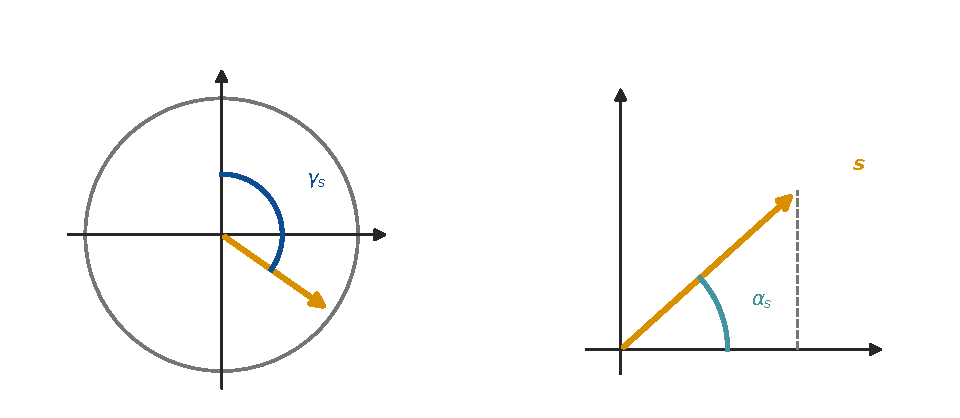
\includegraphics[width=0.94\textwidth]{figures/q1_solar_geometry_cn.pdf}
  \caption{太阳高度角、方位角及太阳中心向量的坐标约定}
  \label{fig:q1-solar-geometry}
\end{figure}

图\ref{fig:q1-solar-geometry}(a)解释了为何方位角必须结合时角确定象限；图\ref{fig:q1-solar-geometry}(b)说明$\sin\alpha_s$就是太阳单位向量的竖直分量。太阳向量既用于后续镜面姿态和阴影光路，也出现在DNI公式中，因此太阳角是整个模型的第一项承重输入。

题目给定海拔$H=3$ km，代入附录参数后，法向直接辐射辐照度为
\begin{equation}
\mathrm{DNI}(t)=1.366\left[0.34981+0.5783875
\exp\left(-\frac{0.275745}{\sin\alpha_s(t)}\right)\right]\ \mathrm{kW/m^2}.
\end{equation}
$\mathrm{DNI}$给出垂直于太阳中心光线平面的能量通量，$\boldsymbol{s}$给出光线方向。余弦效率将在镜面上完成投影，因此不能把DNI再乘一次水平面投影因子。

在把60个状态输入镜场模型之前，需要确认它们都是有效白昼状态，并检查季节和时刻变化是否符合球面几何。图\ref{fig:q1-solar-states}分别给出60个状态的太阳高度角和DNI；每个单元格都对应后续全场计算中的一个时点。

\begin{figure}[H]
  \centering
  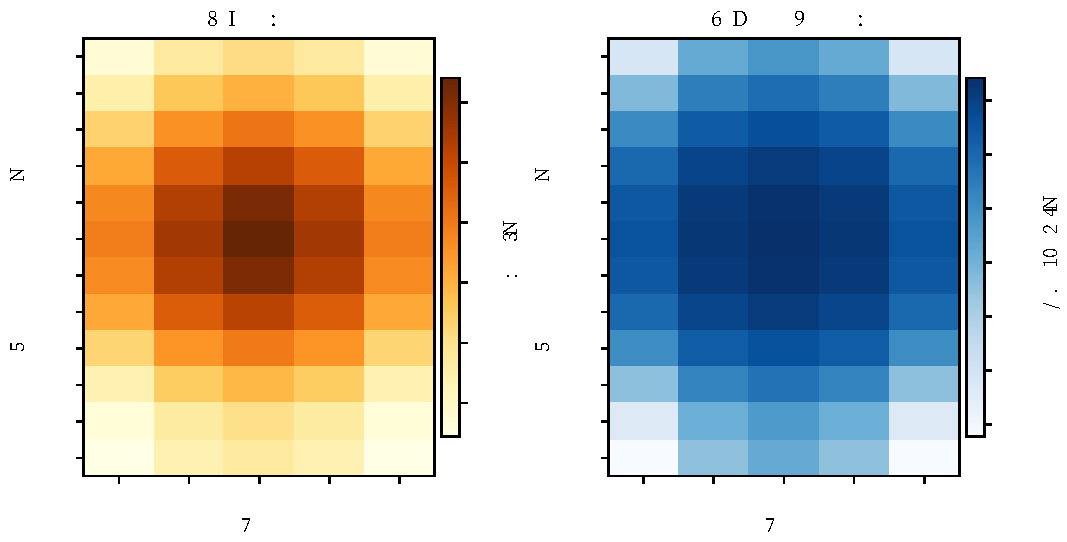
\includegraphics[width=0.98\textwidth]{figures/q1_solar_states_cn.pdf}
  \caption{题目规定60个状态的太阳高度角与法向直接辐射辐照度}
  \label{fig:q1-solar-states}
\end{figure}

图\ref{fig:q1-solar-states}表明60个状态的太阳高度角和DNI均为正；同月内正午最高，同一时刻由冬季向夏季整体升高。上午和下午关于正午具有相同的高度角与DNI，但方位角处于不同象限，所以镜场空间损失仍可能不同，不能只凭DNI对称性推断镜场效率完全对称。

\subsection{步骤二：由反射定律确定镜面姿态}

第$i$面镜的镜心为$\boldsymbol{c}_i=(x_i,y_i,4)^{\mathsf T}$，集热器中心为$\boldsymbol{c}_R=(0,0,76)^{\mathsf T}$。镜心指向集热器中心的单位向量为
\begin{equation}
\boldsymbol{t}_i=\frac{\boldsymbol{c}_R-\boldsymbol{c}_i}
{\|\boldsymbol{c}_R-\boldsymbol{c}_i\|}.
\end{equation}
太阳中心光线的传播方向是$-\boldsymbol{s}$。理想镜面反射算子为
\begin{equation}
\mathcal{R}(\boldsymbol{d},\boldsymbol{n})
=\boldsymbol{d}-2(\boldsymbol{d}\cdot\boldsymbol{n})\boldsymbol{n}.
\end{equation}
控制规则要求$\mathcal{R}(-\boldsymbol{s},\boldsymbol{n}_i)=\boldsymbol{t}_i$，由入射方向与目标方向的角平分关系得到唯一朝阳法向
\begin{equation}
\boldsymbol{n}_i(t)=\frac{\boldsymbol{s}(t)+\boldsymbol{t}_i}
{\|\boldsymbol{s}(t)+\boldsymbol{t}_i\|}.
\end{equation}
该式给出的不是固定安装角，而是随太阳位置更新的目标姿态。对固定的第$i$面镜，$\boldsymbol{t}_i$在一天内保持不变；每到一个计算时点，先更新$\boldsymbol{s}(t)$，再由上式更新$\boldsymbol{n}_i(t)$。因此，同一面镜上午、正午和下午需要转到不同姿态；同一时点的不同镜面也因$\boldsymbol{t}_i$不同而具有不同姿态。

为直观表示控制角，定义法向方位角$\beta_i$从正北顺时针量取，镜面倾角$\tau_i$为镜面平面相对水平面的夹角，则
\begin{equation}
\beta_i(t)=\operatorname{mod}\!\left[
\operatorname{atan2}\bigl(n_{x,i}(t),n_{y,i}(t)\bigr),2\pi\right],
\qquad
\tau_i(t)=\arccos n_{z,i}(t).
\end{equation}
当$\tau_i=0$时镜面水平。这两个角确定题面模型中的目标镜面平面；实际电机轴角还依赖支架零位和传动形式，题面没有提供，故不另行虚构。

以附件第1面镜$\boldsymbol{c}_1=(107.25,11.664,4)^{\mathsf T}$ m为例，图\ref{fig:q1-single-tracking}给出3月21日五个时点的目标姿态。该镜位于塔的东偏北侧，因此即使上午、下午太阳高度角关于正午对称，其镜面姿态也不必关于正午对称。
\begin{figure}[H]
  \centering
  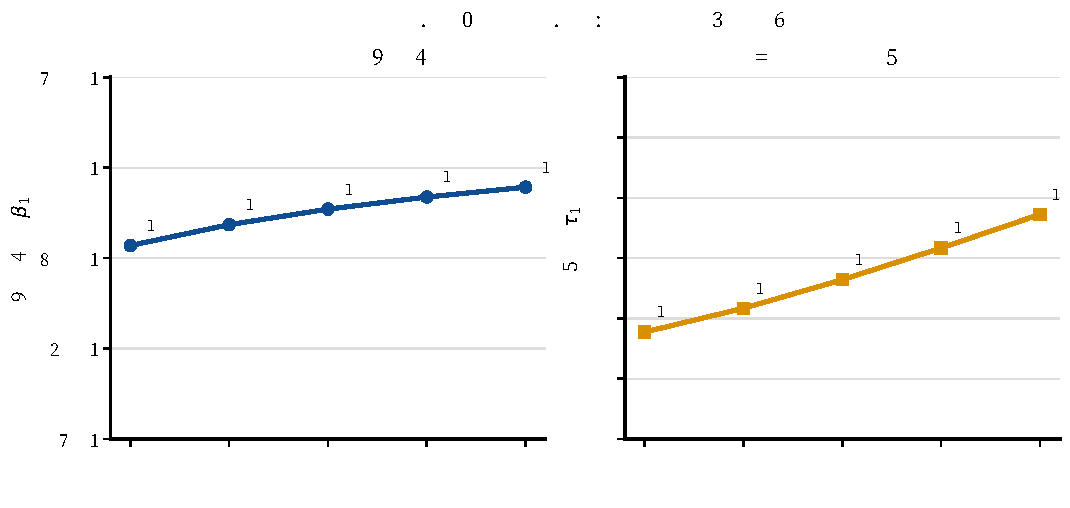
\includegraphics[width=0.92\textwidth]{figures/q1_single_mirror_tracking_cn.pdf}
  \caption{附件第1面定日镜在3月21日的时变目标姿态}
  \label{fig:q1-single-tracking}
\end{figure}

这里“使光线尽量反射至集热器”严格对应题面中心瞄准规则：太阳盘中心光线经镜心反射后指向集热器中心。它不是额外的瞄准点优化，也不意味着太阳锥中的所有边缘光线都必然命中有限接收器；后者仍由截断效率计算。

因此余弦效率是反射几何的解析结果：
\begin{equation}
\eta_{\cos,i}(t)=\boldsymbol{n}_i(t)\cdot\boldsymbol{s}(t)
=\sqrt{\frac{1+\boldsymbol{s}(t)\cdot\boldsymbol{t}_i}{2}}.
\end{equation}

法向只确定镜面所在平面，尚未给出有限矩形边界。令$\boldsymbol{k}=(0,0,1)^{\mathsf T}$，根据“上下边平行地面”的题意构造
\begin{equation}
\boldsymbol{e}_{w,i}=\frac{\boldsymbol{k}\times\boldsymbol{n}_i}
{\|\boldsymbol{k}\times\boldsymbol{n}_i\|},
\qquad
\boldsymbol{e}_{h,i}=\boldsymbol{n}_i\times\boldsymbol{e}_{w,i}.
\end{equation}
于是有限矩形镜面为
\begin{equation}
\mathcal{M}_i(t)=\left\{\boldsymbol{c}_i+u\boldsymbol{e}_{w,i}(t)
+v\boldsymbol{e}_{h,i}(t):u,v\in[-3,3]\right\}.
\end{equation}

这一步需要同时说明反射方向和镜面边界，因为后续光线相交既依赖法向，又必须检查交点是否真正落在$6\ \mathrm{m}\times6\ \mathrm{m}$矩形内部。图\ref{fig:q1-reflection}左图表示法向的角平分关系，右图表示局部宽向、高向和法向如何共同参数化有限镜面。

\begin{figure}[H]
  \centering
  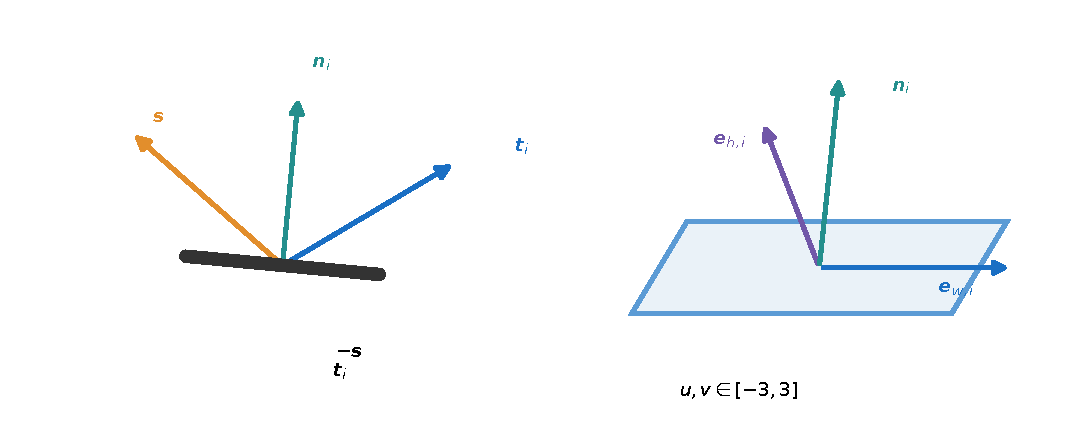
\includegraphics[width=0.98\textwidth]{figures/q1_reflection_geometry_cn.pdf}
  \caption{镜面反射方向、唯一法向与有限矩形局部坐标}
  \label{fig:q1-reflection}
\end{figure}

图\ref{fig:q1-reflection}(a)与法向公式对应：$\boldsymbol{n}_i$位于指向太阳的方向$\boldsymbol{s}$和指向接收器的方向$\boldsymbol{t}_i$之间；图\ref{fig:q1-reflection}(b)与有限镜面参数式对应：只有同时满足$u,v\in[-3,3]$的交点才位于真实镜面上。至此，太阳位置被转换成每个时点、每面镜的唯一三维有限几何对象。

\subsection{步骤三：建立太阳盘方向测度}

题面指出太阳光具有锥形角，说明太阳不能被视为严格单一方向。由于题面没有给出周日比或现场太阳形状，采用经确认的半角$\theta_\odot=4.65\times10^{-3}$ rad均匀pillbox太阳盘。在$\boldsymbol{s}$的正交平面内构造单位基$\boldsymbol{a},\boldsymbol{b}$，太阳盘内方向表示为
\begin{equation}
\boldsymbol{s}'(t,\theta,\psi)=\boldsymbol{s}(t)\cos\theta+
\left[\boldsymbol{a}(t)\cos\psi+\boldsymbol{b}(t)\sin\psi\right]\sin\theta,
\end{equation}
其中$0\le\theta\le\theta_\odot$，$0\le\psi<2\pi$。均匀pillbox是单位立体角内能量相同，因此归一化方向测度为
\begin{equation}
\mathrm{d}\mu_s=\frac{\sin\theta\,\mathrm{d}\theta\,\mathrm{d}\psi}
{2\pi(1-\cos\theta_\odot)}.
\end{equation}
数值采样必须使$\cos\theta$均匀，而不能使$\theta$均匀；否则会过度采样太阳盘中心，系统改变接收器边界附近的命中比例。

镜面法向仍由太阳中心方向确定，但太阳盘内每个方向都要逐条反射：
\begin{equation}
\boldsymbol{r}'_i=-\boldsymbol{s}'+2(\boldsymbol{s}'\cdot\boldsymbol{n}_i)\boldsymbol{n}_i.
\end{equation}
只有$\boldsymbol{s}'=\boldsymbol{s}$时，反射方向才严格等于$\boldsymbol{t}_i$。因此，中心光线命中接收器中心并不能替代对整个太阳锥的有限接收器命中计算。

\subsection{步骤四：在统一光线上定义阴影、遮挡和截断}

对第$i$面镜和时点$t$，定义联合样本空间
\begin{equation}
\Omega_i(t)=\mathcal{M}_i(t)\times\mathcal{S}(t),
\qquad \mathrm{d}\mu_i=\frac{\mathrm{d}A}{A_i}\,\mathrm{d}\mu_s,
\quad A_i=36\ \mathrm{m^2}.
\end{equation}
一个样本$\xi=(\boldsymbol{p},\boldsymbol{s}')$同时指定镜面位置和太阳盘方向，代表一小份确定光路的能量。阴影、遮挡和截断均在同一个联合样本空间上判断，才能保证损失分母一致。

入射阶段从镜面点朝太阳方向回溯：
\begin{equation}
\boldsymbol{q}_{\mathrm{in}}(\lambda)=\boldsymbol{p}+\lambda\boldsymbol{s}',\qquad\lambda>0.
\end{equation}
先定义塔身实体区域
\begin{equation}
\mathcal{C}_T=\{(x,y,z):x^2+y^2\le3.5^2,\ 0\le z<72\}.
\end{equation}
若入射射线不与任何其他有限镜面相交，令$J_i(\xi)=1$，否则为0；若它不与$\mathcal{C}_T$相交，令$T_i(\xi)=1$，否则为0。于是联合入射可见指示量为
\begin{equation}
I_i(\xi)=J_i(\xi)T_i(\xi).
\end{equation}
这样，镜间阴影和塔身阴影在同一条光线上作布尔合并，不会重复扣损。按建模者确认的口径，$72\le z\le80$ m的集热器不作为入射阴影体；该区间只在反射后的接收命中判定中使用。出射阶段沿反射方向追踪
\begin{equation}
\boldsymbol{q}_{\mathrm{out}}(\lambda)=\boldsymbol{p}+\lambda\boldsymbol{r}'_i,\qquad\lambda>0.
\end{equation}
若反射光在到达接收器区域之前先与其他镜面相交，则发生遮挡。定义出射可见指示量$O_i(\xi)$：未被遮挡时取1，否则取0。

阴影和遮挡发生在反射前后不同的有向光段。图\ref{fig:q1-shadow-blocking}分别给出两类光路，以避免把它们混作无方向的平面重叠面积。

\begin{figure}[H]
  \centering
  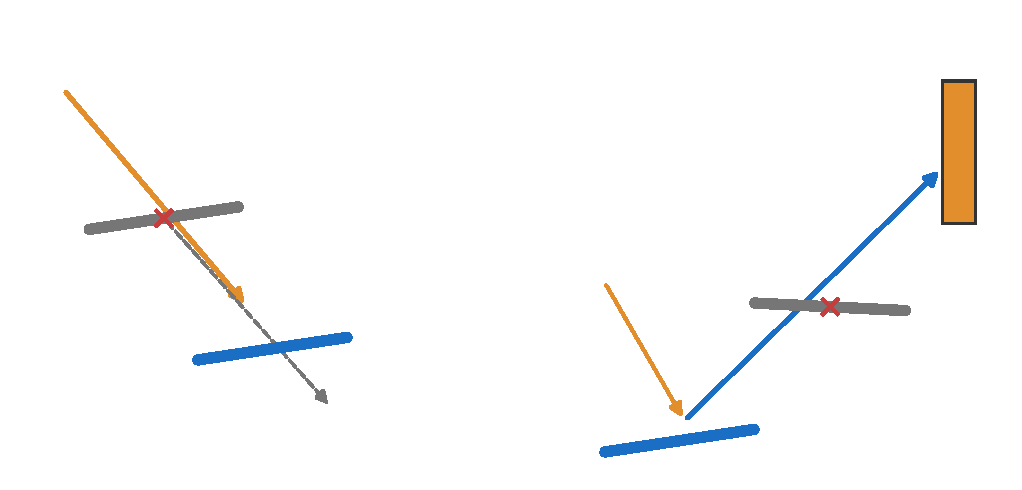
\includegraphics[width=0.98\textwidth]{figures/q1_shadow_blocking_cn.pdf}
  \caption{入射阴影与出射遮挡的有向光路区别}
  \label{fig:q1-shadow-blocking}
\end{figure}

图\ref{fig:q1-shadow-blocking}(a)中光线尚未到达目标镜就与邻镜或塔身相交；图\ref{fig:q1-shadow-blocking}(b)中太阳光已到达目标镜，但反射后在到达接收器前与邻镜相交。程序因此分别沿$+\boldsymbol{s}'$和$+\boldsymbol{r}'$检查正向射线参数，不能用同一个反向投影公式代替两类事件。

接收器有效受光面为
\begin{equation}
\mathcal{C}=\{(x,y,z):x^2+y^2=R^2,\ 72\le z\le80\},\qquad R=3.5\ \mathrm{m}.
\end{equation}
将出射射线代入圆柱方程，得到$a\lambda^2+b\lambda+c=0$，其中
\begin{equation}
a=r_x'^2+r_y'^2,\quad
b=2(p_xr_x'+p_yr_y'),\quad
c=p_x^2+p_y^2-R^2.
\end{equation}
取最小正根$\lambda_R$，再检查$p_z+\lambda_Rr_z'\in[72,80]$。满足时定义命中指示量$H_i(\xi)=1$，否则为0。题面指定外表受光式圆柱，故顶面和底面不计入接收面。

截断损失同时来自太阳盘方向展开和接收器有限直径、高度。图\ref{fig:q1-suncone}先说明太阳盘是一族方向，再说明这族反射光中只有部分命中有限圆柱侧面。

\begin{figure}[H]
  \centering
  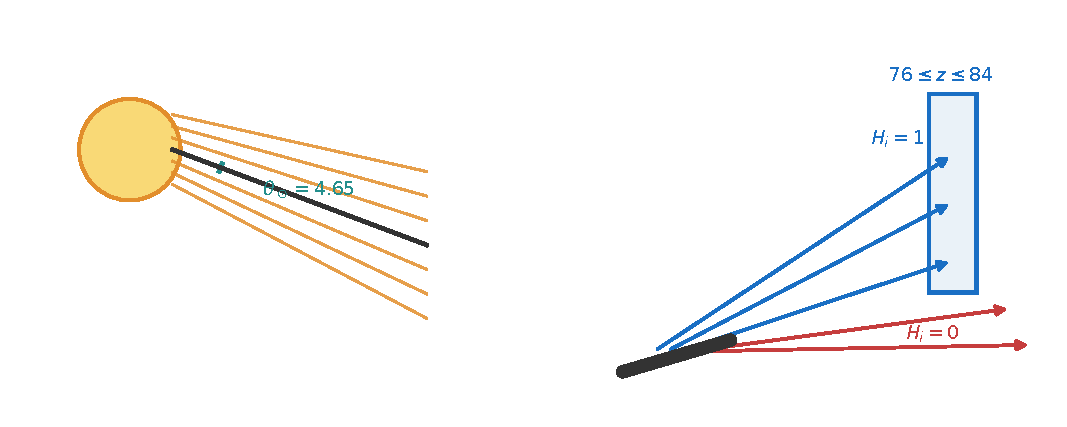
\includegraphics[width=0.98\textwidth]{figures/q1_suncone_receiver_cn.pdf}
  \caption{均匀太阳盘方向与有限圆柱集热器的截断机制}
  \label{fig:q1-suncone}
\end{figure}

图\ref{fig:q1-suncone}(a)对应太阳盘方向测度；图\ref{fig:q1-suncone}(b)对应命中指示量$H_i$。中心光线命中只验证瞄准方向正确，不能说明$\eta_{\mathrm{trunc}}=1$；太阳盘边缘方向和镜面不同位置仍可能形成未命中的反射光。

令光路未受入射阴影和出射遮挡的联合事件为$V_i(\xi)=I_i(\xi)O_i(\xi)$。阴影遮挡效率定义为
\begin{equation}
\eta_{\mathrm{sb},i}(t)=\int_{\Omega_i(t)}V_i(\xi)\,\mathrm{d}\mu_i(\xi).
\end{equation}
题面把截断效率的分母定义为扣除阴影遮挡损失后的反射能量，因此它必须是条件比例：
\begin{equation}
\eta_{\mathrm{trunc},i}(t)=
\frac{\int_{\Omega_i(t)}V_i(\xi)H_i(\xi)\,\mathrm{d}\mu_i(\xi)}
{\int_{\Omega_i(t)}V_i(\xi)\,\mathrm{d}\mu_i(\xi)}.
\end{equation}
于是严格满足
\begin{equation}
\eta_{\mathrm{sb},i}(t)\eta_{\mathrm{trunc},i}(t)
=\int_{\Omega_i(t)}V_i(\xi)H_i(\xi)\,\mathrm{d}\mu_i(\xi).
\end{equation}
右端正是“既未被镜场阻挡，又真正命中接收器”的联合能量比例。该恒等式保证一条光线无论与多少邻镜相交都只记录一次损失，并保证截断效率不使用全部镜面采样作为错误分母。

\subsection{步骤五：从单镜效率到镜场功率}

第$i$面镜到接收器中心的距离为$d_{\mathrm{HR},i}=\|\boldsymbol{c}_R-\boldsymbol{c}_i\|$。附件中全部$d_{\mathrm{HR},i}<1000$ m，故题面大气透射率公式适用：
\begin{equation}
\eta_{\mathrm{at},i}=0.99321-0.0001176d_{\mathrm{HR},i}
+1.97\times10^{-8}d_{\mathrm{HR},i}^2.
\end{equation}
镜面反射率取$\eta_{\mathrm{ref}}=0.92$。单镜综合光学效率为
\begin{equation}
\eta_i(t)=\eta_{\mathrm{sb},i}(t)\eta_{\cos,i}(t)\eta_{\mathrm{at},i}
\eta_{\mathrm{trunc},i}(t)\eta_{\mathrm{ref}}.
\end{equation}
单镜和镜场在时点$t$的输出热功率分别为
\begin{equation}
E_i(t)=\mathrm{DNI}(t)A_i\eta_i(t),
\end{equation}
\begin{equation}
E_{\mathrm{field}}(t)=\sum_{i=1}^{N}E_i(t)
=\mathrm{DNI}(t)\sum_{i=1}^{N}A_i\eta_i(t).
\end{equation}

Q1全部镜面等面积，故时点平均效率可按1745面镜等权：
\begin{equation}
\bar\eta_q(t)=\frac{1}{N}\sum_{i=1}^{N}\eta_{q,i}(t),
\quad q\in\{\mathrm{sb},\cos,\mathrm{trunc},\mathrm{total}\}.
\end{equation}
月平均为当月五个时点的算术平均：
\begin{equation}
\bar\eta_{q,m}=\frac{1}{5}\sum_{h\in\{9,10.5,12,13.5,15\}}\bar\eta_q(m,h),
\end{equation}
题面离散年平均为
\begin{equation}
\bar\eta_{q,\mathrm{year}}=\frac{1}{12}\sum_{m=1}^{12}\bar\eta_{q,m}
=\frac{1}{60}\sum_{t\in\mathcal{T}}\bar\eta_q(t).
\end{equation}

功率也按相同时间权重聚合，但必须先计算每个时点的镜场功率，再求平均：
\begin{equation}
\bar E_{\mathrm{year}}=\frac{1}{60}\sum_{t\in\mathcal{T}}
\mathrm{DNI}(t)\sum_{i=1}^{N}A_i\eta_i(t).
\end{equation}
单位镜面面积年平均输出热功率为
\begin{equation}
P_A=\frac{\bar E_{\mathrm{year}}}{\sum_iA_i}.
\end{equation}
不能用“平均DNI$\times$平均效率”替代上式，因为DNI和光学效率随状态共同变化，两个平均量的乘积一般不等于乘积的平均。

\subsection{连续模型的数值求解}

上述积分包含有限矩形可见性和有限圆柱命中，难以获得闭式解。正式主方法M1分别在镜面局部坐标$(u,v)$和太阳盘立体角上生成随机扰动Sobol低差异样本，再计算两组样本的笛卡尔积。对每个“镜面点--太阳方向”组合依次计算$I_i,O_i,H_i$，用布尔样本均值估计阴影遮挡效率和联合接收比例，最后通过条件关系得到截断效率。

正式细分辨率为64个镜面点与32个太阳方向，共2048条联合光线/镜时种子；固定种子为2023、2024、2025和2026，正式结果取四个细分辨率估计的算术平均。为估计离散误差，同时使用32个镜面点与16个太阳方向的嵌套粗分辨率，相同种子的粗样本是细Sobol序列的前缀。

几何相交只需检查可能影响目标镜的邻镜。程序以镜心平面距离60 m建立候选集，但该剪枝必须与全1745面镜的相交判定进行分层复核。TensorFlow GPU只负责分块执行相同的射线--有限矩形和射线--圆柱求交，不改变物理样本空间或效率定义。

为定位实现错误并量化离散近似影响，另设置可完成全部输出的基线B1。B1在镜面上使用$5\times5$中点网格，以太阳中心方向计算阴影遮挡，再用16个太阳盘方向估计可见网格点的条件截断。B1与M1共享太阳位置、镜面姿态、大气透射、有限圆柱和功率聚合公式，因而二者结果可以直接比较；但B1的低分辨率和因子化近似不用于冻结正式结果。

预定回退规则是：若M1未达到收敛阈值，则将同一方法提高到128个镜面点与64个太阳方向并返回实验判断点；不得把B1自动升级为最终方法。本轮收敛检查通过，故未触发回退。

\subsection{几何验证与数值稳健性}\label{subsec:q1-robustness}

模型验证对应建模链中的具体高风险环节，而不是只检查程序能否运行。除太阳方向、反射方向和集热器命中检查外，还构造了三类塔影案例：入射射线穿过塔身、背离塔身、仅穿过集热器高度区间，预期结果依次为“遮挡、不遮挡、不遮挡”。TensorFlow与NumPy在独立复核案例中的相交计数完全一致；60 m邻镜候选剪枝相对全场判定的阴影遮挡效率最大绝对差为0。

在全部$1745\times60=104700$条逐镜状态记录中，各效率均位于$[0,1]$，未出现NaN或无穷值；联合事件分解的最大残差处于浮点舍入量级，综合效率乘积残差为0，镜场功率与逐镜功率汇总残差为$7.11\times10^{-15}$ MW。这些结果分别验证了太阳角、反射方向、有限边界、条件截断分母和单位聚合。

在把数值写入论文前，还需检查离散分辨率、随机化低差异采样和关键简化假设是否会改变结论。图\ref{fig:q1-robustness}统一使用相对功率变化，并画出预先设置的阈值，避免用截断的绝对功率纵轴夸大小差异。

\begin{figure}[H]
  \centering
  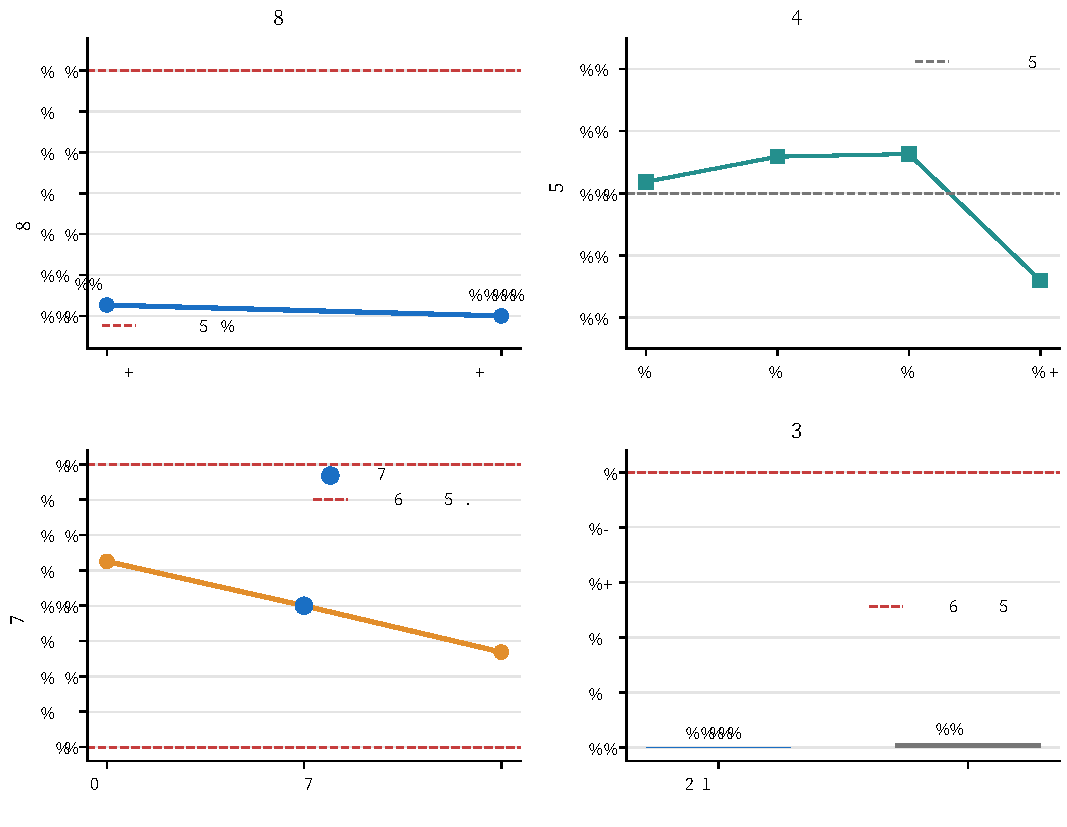
\includegraphics[width=0.98\textwidth]{figures/q1_convergence_robustness_cn.pdf}
  \caption{M1分辨率、固定种子及关键假设的稳健性检查}
  \label{fig:q1-robustness}
\end{figure}

由图\ref{fig:q1-robustness}(a)可见，从$32\times16$提高到$64\times32$后，年平均综合效率的绝对变化为$7.6896\times10^{-5}$，年平均镜场功率相对变化为0.0134\%，12个月单位面积功率的最大相对变化为0.0594\%；三项分别低于0.002、0.3\%和0.5\%阈值。图\ref{fig:q1-robustness}(b)中四种子年平均综合效率标准差为$4.6416\times10^{-5}$，年平均功率极差仅0.007117 MW。

图\ref{fig:q1-robustness}(c)显示，太阳盘半角改变$-5\%$和$+5\%$时，年平均功率分别改变$+0.3140\%$和$-0.3281\%$，均未达到1\%返回决策阈值；太阳锥变宽时反射光斑扩展，功率下降，方向与有限接收器几何一致。图\ref{fig:q1-robustness}(d)显示，按各月天数加权得到34.9918 MW，相对十二个月等权的34.9868 MW仅变化0.0142\%。因此当前分辨率和已批准假设均未触发回退，但这些检查只证明求解器对已定义模型稳定，并不等同于真实电站实测验证。

\subsection{镜场空间分布与月度规律}

全场平均会掩盖不同镜位与太阳时刻的差异。为了说明损失并非一个可对所有镜面套用的常数，图\ref{fig:q1-spatial}先给出附件镜场布局；随后对每面镜的60个规定状态综合效率取等权平均，形成逐镜年均综合光学效率分布；最后选择冬季上午、春季正午和夏季正午三个代表状态展示逐镜瞬时综合效率。年均图与三个时点图使用相同色标，因此既能辨认长期稳定的空间差异，也能直接比较单时点空间不均匀程度。

\begin{figure}[H]
  \centering
  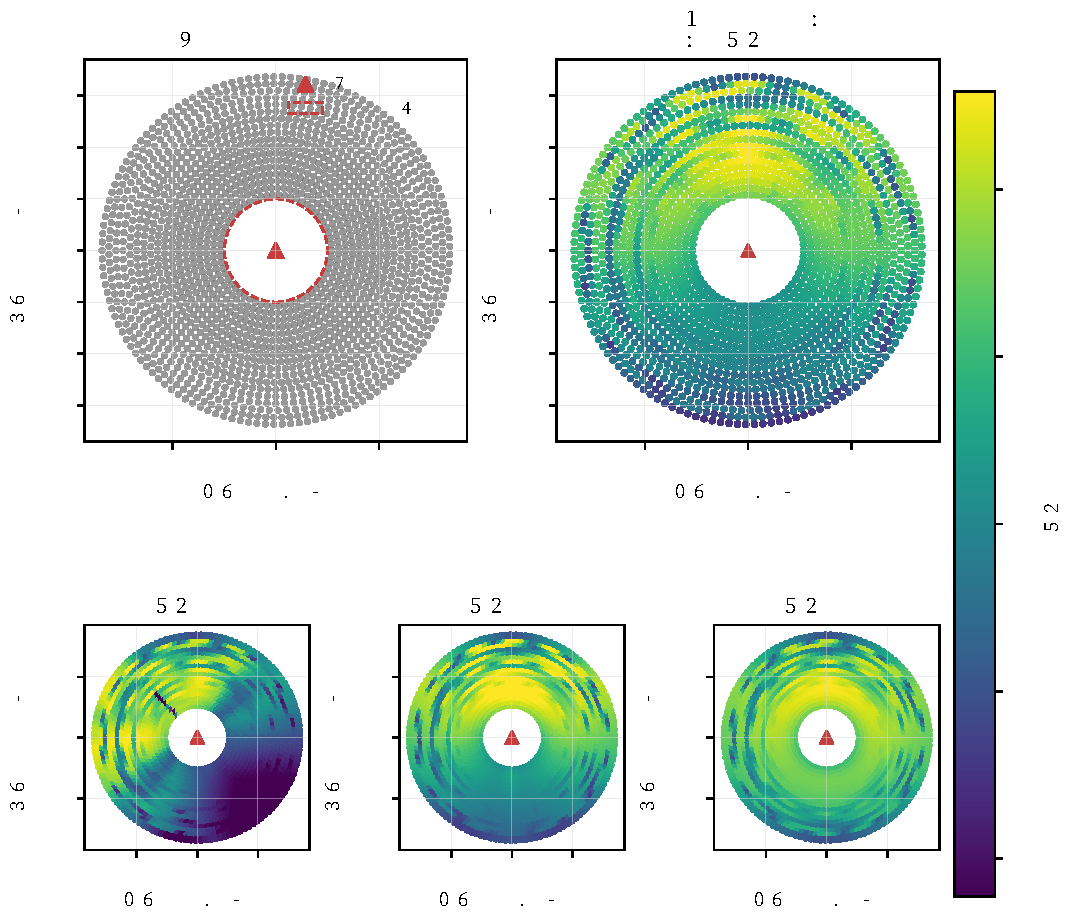
\includegraphics[width=0.98\textwidth]{figures/q1_field_spatial_cn.pdf}
  \caption{镜场布置、逐镜年均综合光学效率与三个代表状态的逐镜综合光学效率}
  \label{fig:q1-spatial}
\end{figure}

图\ref{fig:q1-spatial}(b)给出逐镜年均综合光学效率，它把60个规定状态的短时方向性损失聚合为长期空间差异，可用于识别全年平均意义下持续高效或低效的镜位。图\ref{fig:q1-spatial}(c)表明低太阳高度角下效率具有明显的方向性不均匀，这是余弦方向、镜间遮挡与塔身阴影共同作用的结果；图\ref{fig:q1-spatial}(d)、(e)在正午状态下分布更接近环状，但仍随镜位变化。年均图比单时点更平滑，却没有退化为仅由半径决定的常数，说明必须逐镜、逐时点计算后再聚合，不能只按镜场半径给每面镜赋同一个平均效率。

为把新增的塔身阴影从镜间阴影中单独辨认出来，对第$i$面镜定义60状态累计塔影暴露量
\begin{equation}
N^{\mathrm{eq}}_{T,i}=\sum_{t\in\mathcal{T}}
\Pr_{\boldsymbol{p},\boldsymbol{s}',\mathrm{seed}}
\!\left\{\boldsymbol{q}_{\mathrm{in}}(\lambda)\cap\mathcal{C}_T\neq\varnothing\right\}.
\end{equation}
每个状态中的概率在64个镜面点、32个太阳盘方向和4个固定种子上求平均。因此，$N^{\mathrm{eq}}_{T,i}=1$表示累计塔影暴露量等价于一个规定状态下整面镜完全被塔身遮挡；该量同时反映受影响状态数和每个状态的遮挡面积比例，但不混入镜间阴影。

\begin{figure}[H]
  \centering
  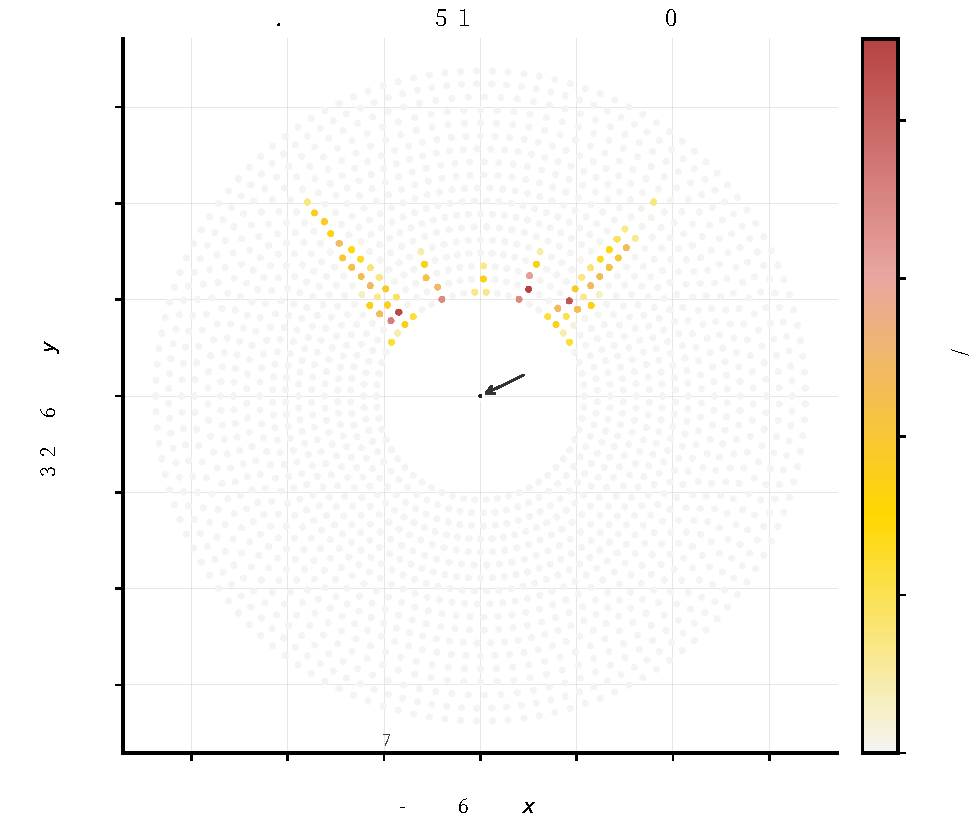
\includegraphics[width=0.92\textwidth]{figures/q1_tower_shadow_exposure_cn.pdf}
  \caption{60个规定太阳状态叠加的定日镜塔身阴影暴露分布}
  \label{fig:q1-tower-shadow}
\end{figure}

图\ref{fig:q1-tower-shadow}中颜色越深，表示累计塔影暴露越强。共有72面定日镜出现非零塔影，单镜最大累计暴露为2.2574个等效状态。受影响镜面主要位于塔的北侧，并向西北和东北展开，这是因为规定时点的太阳位于南侧天空，塔影总体投向北方，而上午、下午太阳方位变化使阴影方向分别发生横向偏转。这里的“全年叠加”特指题目规定60个状态的等权累计，不等同于真实全年逐分钟遮挡时长。

月度功率同时受到DNI、余弦效率、阴影遮挡效率、截断效率和大气透射率影响。因此，图\ref{fig:q1-monthly}左侧同时展示主要效率分量，右侧展示最终单位面积功率，避免把季节变化错误归因于单一因素。

\begin{figure}[H]
  \centering
  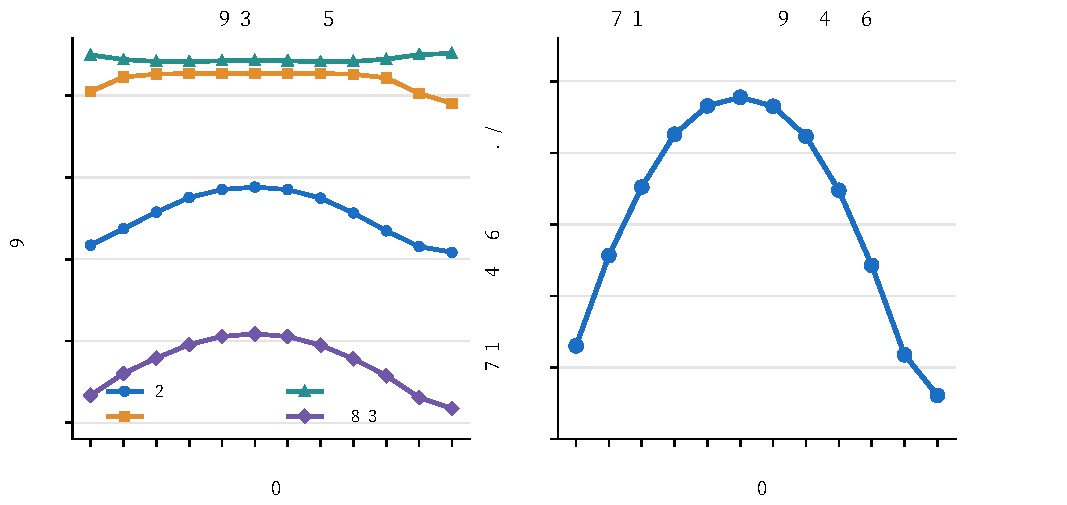
\includegraphics[width=0.98\textwidth]{figures/q1_monthly_results_cn.pdf}
  \caption{月平均光学效率分解与单位镜面面积输出热功率}
  \label{fig:q1-monthly}
\end{figure}

图\ref{fig:q1-monthly}显示，余弦效率和阴影遮挡效率由冬季向夏季上升，再向冬季下降；截断效率全年均高于0.941，变化较小且冬季略高，但不能抵消冬季较低的DNI、余弦效率和阴影遮挡效率。单位面积月平均输出热功率在6月达到最高值0.6388 kW/m$^2$，在12月达到最低值0.4306 kW/m$^2$，整体呈冬低夏高的规律。

\subsection{题目要求的月度与年度结果}

表\ref{tab:q1-monthly}给出题目表1所需的12个月结果。效率和单位面积输出热功率均保留4位小数；所有显示值都由冻结的正式结果统一四舍五入，未进行人工调整。

\begin{table}[H]
\centering
\small
\setlength{\tabcolsep}{4.2pt}
\caption{问题一每月平均光学效率及单位面积输出热功率}
\label{tab:q1-monthly}
\begin{tabular}{cccccc}
\toprule
月份 & 综合效率 & 余弦效率 & 阴影遮挡效率 & 截断效率 & 单位面积功率/(kW/m$^2$)\\
\midrule
1  & 0.5336 & 0.7171 & 0.9048 & 0.9497 & 0.4652\\
2  & 0.5603 & 0.7372 & 0.9227 & 0.9441 & 0.5283\\
3  & 0.5792 & 0.7575 & 0.9262 & 0.9417 & 0.5761\\
4  & 0.5956 & 0.7754 & 0.9269 & 0.9414 & 0.6130\\
5  & 0.6056 & 0.7852 & 0.9271 & 0.9426 & 0.6328\\
6  & 0.6088 & 0.7881 & 0.9273 & 0.9431 & 0.6388\\
7  & 0.6054 & 0.7851 & 0.9271 & 0.9425 & 0.6325\\
8  & 0.5949 & 0.7747 & 0.9269 & 0.9414 & 0.6116\\
9  & 0.5782 & 0.7565 & 0.9261 & 0.9417 & 0.5739\\
10 & 0.5576 & 0.7347 & 0.9216 & 0.9445 & 0.5215\\
11 & 0.5309 & 0.7154 & 0.9026 & 0.9501 & 0.4589\\
12 & 0.5174 & 0.7085 & 0.8906 & 0.9516 & 0.4306\\
\bottomrule
\end{tabular}
\end{table}

表\ref{tab:q1-annual}给出题目表2所需的年度指标。年平均镜场输出热功率为34.9868 MW；除以总镜面面积62820 m$^2$后，单位面积年平均输出热功率为0.5569 kW/m$^2$。两者由同一时点功率链条聚合，单位换算相互一致。

\begin{table}[H]
\centering
\small
\caption{问题一题面离散年平均光学效率及输出热功率}
\label{tab:q1-annual}
\begin{tabular}{lcc}
\toprule
指标 & 数值 & 单位\\
\midrule
年平均综合光学效率 & 0.5723 & --\\
年平均余弦效率 & 0.7529 & --\\
年平均阴影遮挡效率 & 0.9192 & --\\
年平均截断效率 & 0.9445 & --\\
年平均镜场输出热功率 & 34.9868 & MW\\
单位面积年平均输出热功率 & 0.5569 & kW/m$^2$\\
\bottomrule
\end{tabular}
\end{table}

为说明数值离散口径的影响，表\ref{tab:q1-baseline}给出M1与B1的年度对照。二者余弦效率完全一致，因为都使用解析太阳角和镜面法向；B1的综合效率比M1高0.0059，年平均功率高0.3639 MW，差异主要来自低分辨率因子化近似对阴影遮挡和截断边界的处理。

\begin{table}[H]
\centering
\small
\caption{M1正式主方法与B1可用基线的年度结果对照}
\label{tab:q1-baseline}
\begin{tabular}{lccc}
\toprule
指标 & M1主方法 & B1基线 & 绝对差\\
\midrule
综合光学效率 & 0.5723 & 0.5782 & 0.0059\\
余弦效率 & 0.7529 & 0.7529 & 0.0000\\
阴影遮挡效率 & 0.9192 & 0.9206 & 0.0015\\
截断效率 & 0.9445 & 0.9523 & 0.0077\\
镜场输出热功率/MW & 34.9868 & 35.3507 & 0.3639\\
单位面积功率/(kW/m$^2$) & 0.5569 & 0.5627 & 0.0058\\
\bottomrule
\end{tabular}
\end{table}

该对照不把M1与B1的差值解释为相对于真实镜场的测量误差。M1作为正式结果的依据是：它直接估计经确认的连续联合光线模型，并通过了物理恒等式、嵌套分辨率和多种子检查；B1只保留为可用回归基线。

\subsection{本问结论与局限}

本问建立了从太阳位置、理想镜面反射、有限矩形镜间相交、塔身圆柱阴影到有限圆柱接收的统一光学模型。其关键不是简单相乘各项平均效率，而是在同一镜面点和太阳盘方向上定义阴影、遮挡与接收事件，使$\eta_{\mathrm{sb}}\eta_{\mathrm{trunc}}$严格等于未受阻挡且命中接收器的联合能量比例；随后逐镜、逐时点计算功率，再按题面权重聚合。

在题目规定的60个代表状态、1745面理想平面镜、72 m圆柱塔身和半角4.65 mrad均匀pillbox太阳盘下，年平均综合光学效率为0.5723，年平均镜场输出热功率为34.9868 MW，单位镜面面积年平均输出热功率为0.5569 kW/m$^2$。嵌套分辨率、四个固定种子、太阳盘半角和月份权重检查均未触发回退阈值。

模型的限制也必须保留：60状态离散平均不能替代真实逐日气象积分；理想镜面假设未包含面形、斜率、跟踪和污染损失；均匀pillbox未描述缺少参数依据的周日区；题面功率公式也没有包含接收器吸收与热损失。因此，本问结果适用于题面定义的光学评价与后续优化统一内核，不应直接外推为真实电站净发电量。

\section{问题二：统一规格定日镜场优化设计}
\subsection{设计变量与目标}
问题二的设计变量包括吸收塔平面坐标$(x_T,y_T)$、统一镜宽$w$、镜高$h$、安装高度$z_H$、镜面总数$N$和各镜心坐标$(x_i,y_i)$。以总镜面面积
\[
A_{\mathrm{tot}}=Nwh
\]
为面积基准，单位镜面面积年平均输出可写为
\[
P_A=\frac{\overline{E}_{\mathrm{field}}}{A_{\mathrm{tot}}}.
\]
目标是在满足额定功率与全部几何规则的条件下使$P_A$尽量大。

\subsection{约束接口}
候选设计至少须通过以下检查：
\begin{enumerate}[itemindent=2em]
  \item 年平均输出热功率$\overline{E}_{\mathrm{field}}\geq60$ MW，并保留足以覆盖复算误差的裕量；
  \item 镜面宽高均在$[2,8]$ m内，且$w\geq h$；
  \item 安装高度在$[2,6]$ m内，并满足完整旋转包络不触地；
  \item 镜场满足建设区域边界、塔周100 m禁布区和相邻镜间距约束。
\end{enumerate}

\subsection{求解、验证与结果}
\pending{写入人类批准的主方法与可用基线、候选表示、约束处理和停止条件。}

\pending{写入风险探针、基线比较、功率裕量、扰动敏感性、固定随机种子及最终高精度复算。}

\pending{从冻结数值生成问题二表1至表3和\path{result2.xlsx}，并验证论文与Excel逐字段一致。}

\section{问题三：可变规格定日镜场优化设计}

\subsection{问题扩展与优化目标}

问题二要求全场镜面规格统一，问题三则允许每面定日镜分别选择宽度、高度和安装高度，并允许重新确定吸收塔位置、镜面总数和全部镜位。新增自由度可以缩小低贡献镜面以减少总面积，也可以调整安装高度以改善遮挡关系；但镜面尺寸一旦变化，最小间距、镜面面积和逐镜光学效率会同时变化。因此，本问不能在问题二镜场上只替换少量规格，而应把布局生成与逐镜规格优化统一起来。

设吸收塔平面坐标为$(x_T,y_T)$，第$i$面定日镜的镜心为$(x_i,y_i,z_i)$，宽度、高度和面积分别为$w_i,h_i$和$a_i=w_ih_i$，镜面总数为$N$。第$k$个规定太阳状态的法向直接辐射强度为$D_k$，问题一光学模型计算的第$i$面镜总光学效率为$\eta_{ik}$。该时刻镜场输出热功率为
\begin{equation}
 P_k=10^{-3}D_k\sum_{i=1}^{N}a_i\eta_{ik}.
 \label{eq:q3-state-power}
\end{equation}
式中的$10^{-3}$将DNI与镜面面积相乘所得的kW换算为MW。
对题目规定的12个月、每月5个时刻作等权平均，得到年平均输出热功率
\begin{equation}
 \overline P=\frac{1}{60}\sum_{k=1}^{60}P_k.
 \label{eq:q3-annual-power}
\end{equation}
总镜面面积和单位面积年平均输出热功率为
\begin{equation}
 A_{\mathrm{tot}}=\sum_{i=1}^{N}w_ih_i,
 \qquad
 P_A=\frac{1000\overline P}{A_{\mathrm{tot}}}\quad(\mathrm{kW/m^2}).
 \label{eq:q3-unit-power}
\end{equation}
式\eqref{eq:q3-unit-power}中的1000用于将MW换算为kW。由此，本问的目标不是无约束地增加总功率，而是在年平均功率达到60 MW后最大化$P_A$：
\begin{equation}
 \max_{\mathcal D_3}\quad P_A,
 \qquad
 \mathrm{s.t.}\quad \overline P\ge60\ \mathrm{MW},
 \label{eq:q3-objective}
\end{equation}
其中
\[
 \mathcal D_3=\left\{x_T,y_T,N,(x_i,y_i,z_i,w_i,h_i)_{i=1}^{N}\right\}.
\]
容量约束负责筛除总面积过小的高效率方案，$P_A$负责比较达到容量要求后的镜场。二者次序不能互换，否则优化器会偏向面积很小但总功率不足的镜场。

当各镜面积不同时，镜场平均效率必须与式\eqref{eq:q3-state-power}保持一致。对余弦、阴影遮挡、截断等任一效率分量$q$，本文采用面积加权
\begin{equation}
 \overline\eta_{q,k}
 =\frac{\sum_{i=1}^{N}a_i\eta_{q,ik}}{A_{\mathrm{tot}}}.
 \label{eq:q3-area-weighted-efficiency}
\end{equation}
若使用逐镜等权，小尺寸镜面会获得与大尺寸镜面相同的权重，所得平均效率将不能还原实际功率，故不采用该口径。

\subsection{逐镜几何约束}

吸收塔和镜心须位于半径350 m的建设圆内，镜心须处于以吸收塔为圆心、半径100 m的禁布区外，即
\begin{equation}
 x_T^2+y_T^2\le350^2,\qquad
 x_i^2+y_i^2\le350^2,\qquad
 (x_i-x_T)^2+(y_i-y_T)^2\ge100^2.
 \label{eq:q3-site-constraints}
\end{equation}
第$i$、$j$面镜的宽度不同时，镜心间距采用两镜宽度半和加5 m：
\begin{equation}
 \sqrt{(x_i-x_j)^2+(y_i-y_j)^2}
 \ge\frac{w_i+w_j}{2}+5,qquad i\ne j.
 \label{eq:q3-heterogeneous-spacing}
\end{equation}
该式在$w_i=w_j$时退化为问题二的$d_{ij}\ge w+5$，因而两问口径一致。程序利用空间索引搜索所有可能冲突的近邻对，再按式\eqref{eq:q3-heterogeneous-spacing}逐对检查，分区边界上的镜对也包含在内。

根据题目边界和镜面宽度一般不小于高度的要求，每面镜满足
\begin{equation}
 2\le h_i\le w_i\le8,qquad 2\le z_i\le6.
 \label{eq:q3-size-constraints}
\end{equation}
为保证镜面转动时不接触地面，以半镜高构造保守旋转包络：
\begin{equation}
 z_i-\frac{h_i}{2}>0.
 \label{eq:q3-ground-clearance}
\end{equation}
综上，式\eqref{eq:q3-objective}与式\eqref{eq:q3-site-constraints}--\eqref{eq:q3-ground-clearance}构成连续规格、离散镜数和非光滑光学效率耦合的约束优化模型。

\subsection{连续布局生成与遗传搜索}

若把2939面左右定日镜的全部镜位和规格直接编码，变量数接近$5N$，有限预算内难以形成有效群体搜索。因此，第一层不直接移动每个镜心，而是用少量连续参数生成完整合法镜场。考虑圆形场界和密排需求，采用两径向区三角晶格。内、外区可以具有不同基础尺寸、相位和高宽比，所有候选均从空场重新生成，不继承问题二坐标。

遗传算法个体编码为
\begin{equation}
 \boldsymbol\theta=
 (y_T,R_b,w_{\mathrm{in}},w_{\mathrm{out}},
 \phi_{\mathrm{in}},\phi_{\mathrm{out}},
 \rho_{\mathrm{in}},\rho_{\mathrm{out}},c),
 \label{eq:q3-ga-vector}
\end{equation}
其中$R_b$为两区径向分界，$\rho=h/w$为高宽比，$c$为离地净空参数。$\phi$表示三角点阵的\textbf{纵向平移相位}，不是点阵旋转角。具体地，对内区或外区$q\in\{\mathrm{in},\mathrm{out}\}$，令最近邻间距和相邻行距分别为
\begin{equation}
 d_q=w_q+5,\qquad \Delta y_q=\frac{\sqrt{3}}{2}d_q,
\end{equation}
则该区三角点阵第$m$行、第$n$列的母池坐标可写为
\begin{equation}
 y_{q,m}=y_T+(m+\phi_q)\Delta y_q,\qquad
 x_{q,mn}=\left[n+\frac{1}{2}(m\bmod 2)\right]d_q.
 \label{eq:q3-lattice-phase}
\end{equation}
因此，$\phi_q\in[0,1)$只使该区全部点阵行沿$y$方向平移$\phi_q\Delta y_q$，不改变最近邻距离、交错结构和点阵方向。例如，$\phi_q=0.5$表示整体平移半个行距。引入该变量是为了调整点阵行与塔周禁布圆、径向分区边界及另一分区点阵的相对位置，从而允许镜面数量和合法镜位随布局连续变化。连续搜索范围为
\begin{equation}
\begin{aligned}
 &y_T\in[-120,20],\quad R_b\in[120,320],\\
 &w_{\mathrm{in}},w_{\mathrm{out}}\in[2,8],\\
 &\phi_{\mathrm{in}},\phi_{\mathrm{out}}\in[0,0.99],\\
 &\rho_{\mathrm{in}},\rho_{\mathrm{out}}\in[0.85,1],
 \quad c\in[0.5,0.9].
\end{aligned}
 \label{eq:q3-ga-bounds}
\end{equation}
上述变量全部采用浮点实数编码。初始化时设置少量边界覆盖点，是为了避免初始种群遗漏$2$ m和$8$ m附近区域；交叉和变异仍在式\eqref{eq:q3-ga-bounds}的整个连续区间内进行，并非只在若干离散尺寸中选择。

对每个个体，先按两区参数生成候选三角晶格点，再依次执行场界、禁布区和异尺寸间距检查，只有合法镜面才被接纳。镜面总数$N$由基础尺寸、区界、相位、塔位和场界共同产生，故随个体自然变化。本轮14个体迭代5代，共完成70次布局评价，实际镜数覆盖2498至7128面，说明搜索确实改变了镜面数量与位置。

候选评价采用容量优先的约束排序。未达到安全功率阈值时，优先提高$\overline P$；达到阈值后，再按$P_A$排序。搜索层使用覆盖四季和不同太阳高度的代表状态进行快速淘汰，前列非重复候选再用全部60状态和$8\times4$光线样本复核。

\subsection{逐镜连续细化与容量修复}

外层搜索得到的候选布局含2939面镜，吸收塔纵坐标约为$-37.43$ m。随后固定镜心坐标，先连续优化安装高度，再计算每面镜的年均单位面积光学贡献。低贡献镜面优先进入规格调整集合，由差分进化搜索受调镜比例、贡献排序指数和宽高缩减尺度；最终变化量落实到每面镜的连续$w_i,h_i,z_i$。每次接受新阶段前均重新检查式\eqref{eq:q3-site-constraints}--\eqref{eq:q3-ground-clearance}，并要求单位面积功率提高且中精度总功率保持在容量安全带内。

逐镜细化的前三阶段分别得到60.3442、60.2211和60.1485 MW的单种子$8\times4$功率，单位面积功率依次提高到0.4532、0.4555和0.4568 kW/m$^2$。然而，第三阶段在$16\times8$、$32\times16$和四种子正式复核下只有59.9052 MW。该结果说明：当候选逼近60 MW边界时，中精度采样的乐观误差足以改变可行性，不能因单位面积指标更高而保留该方案。

为在相同镜数和镜位上恢复正式容量裕量，设第一、第二连续细化阶段的逐镜参数分别为$\boldsymbol v_i^{(1)}=(z_i^{(1)},w_i^{(1)},h_i^{(1)})$和$\boldsymbol v_i^{(2)}$，采用
\begin{equation}
 \boldsymbol v_i=(1-\alpha)\boldsymbol v_i^{(1)}
 +\alpha\boldsymbol v_i^{(2)},\qquad \alpha=0.2.
 \label{eq:q3-capacity-repair}
\end{equation}
式\eqref{eq:q3-capacity-repair}在两组合法连续规格之间插值，并不把镜面恢复为少数标准尺寸。它适度增加总面积，以牺牲部分$P_A$换取正式功率裕量。插值方案经完整复核后满足全部约束，因此作为最终方案。

\subsection{优化结果}

最终吸收塔坐标为$(0,-37.4265)$ m，共布置2939面定日镜，总镜面面积132952.1202 m$^2$。镜宽为4.7554--6.8000 m，镜高为4.7482--6.8000 m，安装高度为3.4091--4.8225 m。六位小数口径下分别有205种镜宽、205种镜高和2512种安装高度，说明最终结果保留了逐镜连续规格，而非退化为两三种离散镜面。

\begin{table}[htbp]
  \centering
  \caption{问题三各月平均光学效率及输出热功率}
  \label{tab:q3-monthly}
  \scriptsize
  \setlength{\tabcolsep}{2.1pt}
  \begin{tabular}{c*{5}{c}@{\hspace{5pt}}c*{5}{c}}
    \toprule
    月 & $\eta$ & $\eta_{\mathrm{cos}}$ & $\eta_{\mathrm{sb}}$ & $\eta_{\mathrm{trunc}}$ & $P_A$
    & 月 & $\eta$ & $\eta_{\mathrm{cos}}$ & $\eta_{\mathrm{sb}}$ & $\eta_{\mathrm{trunc}}$ & $P_A$ \\
    \midrule
    1 & 0.4228 & 0.7458 & 0.7185 & 0.9375 & 0.3693 & 7  & 0.4934 & 0.7904 & 0.7818 & 0.9126 & 0.5155 \\
    2 & 0.4598 & 0.7608 & 0.7655 & 0.9253 & 0.4337 & 8  & 0.4870 & 0.7854 & 0.7809 & 0.9133 & 0.5006 \\
    3 & 0.4766 & 0.7749 & 0.7795 & 0.9159 & 0.4741 & 9  & 0.4761 & 0.7742 & 0.7793 & 0.9163 & 0.4724 \\
    4 & 0.4873 & 0.7858 & 0.7809 & 0.9131 & 0.5015 & 10 & 0.4562 & 0.7589 & 0.7613 & 0.9266 & 0.4268 \\
    5 & 0.4935 & 0.7904 & 0.7819 & 0.9126 & 0.5157 & 11 & 0.4185 & 0.7444 & 0.7130 & 0.9383 & 0.3626 \\
    6 & 0.4955 & 0.7915 & 0.7823 & 0.9128 & 0.5199 & 12 & 0.3993 & 0.7390 & 0.6882 & 0.9406 & 0.3335 \\
    \bottomrule
  \end{tabular}
  \\[2pt]
  \footnotesize 注：$P_A$的单位为kW/m$^2$，其余各列均为无量纲效率。
\end{table}

表\ref{tab:q3-monthly}给出题目表1所需的12个月结果。冬季太阳高度较低，阴影遮挡效率下降，单位面积功率相应较小；5--7月太阳高度较高，阴影遮挡损失减弱，单位面积功率达到全年较高水平。该解释只描述题目60个规定状态下的季节变化，不外推到未计算的逐日运行条件。

\begin{table}[htbp]
  \centering
  \caption{问题三年平均效率与输出热功率}
  \label{tab:q3-annual}
  \small
  \setlength{\tabcolsep}{5pt}
  \begin{tabular}{cccccc}
    \toprule
    指标 & 数值 & 指标 & 数值 & 指标 & 数值 \\
    \midrule
    光学效率 & 0.4639 & 余弦效率 & 0.7701 & 阴影遮挡效率 & 0.7594 \\
    截断效率 & 0.9221 & 输出热功率 & 60.1119 MW & 单位面积功率 & 0.4521 kW/m$^2$ \\
    \bottomrule
  \end{tabular}
\end{table}

\begin{table}[htbp]
  \centering
  \caption{问题三最终设计参数与连续规格范围}
  \label{tab:q3-design}
  \small
  \setlength{\tabcolsep}{6pt}
  \begin{tabular}{cccc}
    \toprule
    参数 & 最终值 & 参数 & 最终值 \\
    \midrule
    吸收塔坐标 & $(0,-37.4265)$ m & 定日镜总数 & 2939面 \\
    定日镜总面积 & 132952.1202 m$^2$ & 最小离地净空 & 0.0500 m \\
    镜面宽度范围 & 4.7554--6.8000 m & 镜面高度范围 & 4.7482--6.8000 m \\
    安装高度范围 & 3.4091--4.8225 m & 连续规格种类 & 205/205/2512种$^{*}$ \\
    \bottomrule
  \end{tabular}
  \\[2pt]
  \footnotesize 注：$^{*}$依次为六位小数口径下的镜宽、镜高和安装高度种类数。
\end{table}

与问题二同一光学和数值口径下的统一规格方案相比，问题三单位面积功率由0.447156 kW/m$^2$提高到0.452132 kW/m$^2$，相对提高1.1127\%；总面积减少约1286.59 m$^2$，而正式年平均功率仍达到60.111866 MW。该比较支持异质规格在已搜索布局族中能够削减低贡献面积并维持容量，但不等同于对所有可能自由布局的全局最优证明。

\subsection{正式复核与结果边界}

正式评价使用全部60个太阳状态。镜面位置与太阳盘方向的联合采样先采用$16\times8$分辨率，再提升至$32\times16$；年平均功率相对变化为0.0450\%，12个月单位面积功率的最大相对变化为0.1413\%，数值收敛判定通过。

在种子2023、2024、2025和2026下，细分辨率年平均功率依次为60.0805、60.1070、60.1260和60.1340 MW，标准差为0.0206 MW，四个结果均满足60 MW。全场2939面镜均位于建设场界内和禁布区外，异尺寸间距违规数为0，$h_i>w_i$违规数为0，最小离地净空为0.05 m。

最终池化功率相对60 MW的裕量为0.1119 MW，最小种子裕量为0.0805 MW。该裕量足以通过本文的数值采样检验，但尚未包含镜面制造误差、跟踪误差、地形起伏和长期污染等工程不确定性。因此，本文把该方案表述为给定物理模型、连续参数化布局族和记录搜索预算下的最佳已验证可行方案，不宣称其为全部逐镜自由设计中的全局最优。全部镜面坐标、宽度、高度和安装高度见提交文件\path{result3.xlsx}。

\section{模型分析与评价}

\subsection{模型的整体结构}

三个问题共用同一套太阳位置、镜面跟踪、光线反射和损失计算模型，区别只在于待求变量逐步增加。问题一在给定镜场上完成光学性能评价，为后续优化提供统一的目标函数与约束判定器；问题二在统一镜面规格条件下联合搜索塔位、布局和镜面尺寸；问题三进一步开放逐镜宽度、高度和安装高度，并以面积加权方式计算异质镜场功率。这样的递进结构保证了三问数值能够在同一物理口径下比较，也避免在优化阶段使用与评价阶段不一致的近似指标。

\subsection{模型优点}

首先，模型保持了从太阳矢量到接收器命中的完整几何链条。每面定日镜均依据入射方向和指向接收器中心的方向实时确定法向量，余弦损失、阴影遮挡、大气透射和截断损失均在同一光线样本上计算，因此各效率分量与最终功率之间具有明确对应关系。对于问题三的异质镜面，采用镜面面积加权而非逐镜等权，使效率汇总能够严格还原功率计算式。

其次，优化过程把容量约束置于单位面积功率比较之前。问题二和问题三均先要求年平均输出热功率不低于60 MW，再最大化单位镜面面积年平均输出热功率，从而排除了面积很小、效率较高但不能完成供热任务的伪优方案。场界、禁布区、异尺寸间距、宽高关系及离地净空均在候选生成和正式复核阶段再次检查，使所得方案同时满足光学目标和几何可实施条件。

最后，模型采用分层精度控制搜索误差。低分辨率用于大范围筛选，高分辨率和多随机种子只用于候选复核。问题一的分辨率与随机种子检验表明评价结果较为稳定；问题二、问题三的最终方案也均经过两级分辨率和四种子检验。问题三细化过程中还主动剔除了在高分辨率下跌破60 MW的候选，说明容量判定以正式复核结果为准，而不是以搜索阶段的乐观估计为准。

\subsection{模型局限与改进方向}

本文结论适用于题目给定的60个离散太阳状态及所建立的理想化光学模型。太阳盘采用均匀pillbox角分布，尚未引入周日亮度、镜面斜率误差、跟踪误差和长期积灰；接收器按几何命中统计截断效率，也未进一步模拟接收器表面热流密度与热损失。因此，所得功率表示规定状态下的光学输出，不应直接解释为包含天气和设备可用率的实际电站年发电量。

此外，问题二和问题三含有离散镜数、非光滑遮挡关系及大量连续变量，粒子群、遗传算法与差分进化给出的是记录搜索范围和预算下的最佳已验证可行解，而非数学意义上的全局最优解。特别是两问的容量裕量均较小，工程设计时还需为制造、跟踪和气象不确定性预留更大的安全裕度。后续可引入实测DNI权重、非均匀太阳形状和误差卷积，并把接收器峰值热流及容量裕量纳入稳健多目标优化，以提高工程适用性。

\section{总结}

本文建立了由太阳位置、双向量定日镜跟踪、光线级阴影遮挡与截断判定组成的统一光学模型，并据此完成给定镜场评价、统一规格镜场优化和逐镜连续规格优化。

对于问题一，给定镜场在题目60个太阳状态下的年平均光学效率为0.5723，年平均输出热功率为34.9868 MW，单位镜面面积年平均输出热功率为0.5569 kW/m$^2$。对于问题二，最密三角晶格与分区参数化搜索得到满足60 MW约束的统一规格方案，其年平均输出热功率为60.0257 MW，单位面积功率为0.4472 kW/m$^2$。对于问题三，从空场重新生成布局并连续调整逐镜宽度、高度和安装高度后，最终2939面定日镜的总面积为132952.1202 m$^2$，年平均输出热功率为60.1119 MW，单位面积功率达到0.4521 kW/m$^2$，较问题二提高1.1127\%。

综合三问可见，在相同光学评价口径下，参数化密排能够控制大规模镜位搜索的计算量，逐镜连续规格则能进一步削减低贡献镜面面积。最终结果均通过分辨率和多随机种子复核，但其有效范围仍受离散太阳状态、理想化太阳盘以及未计入工程误差等假设限制，因而应将其理解为本文模型与搜索预算下的可行设计结果。


\clearpage
\begin{thebibliography}{9}
\bibitem{cumcm2023a}
全国大学生数学建模竞赛组委会.
2023高教社杯全国大学生数学建模竞赛A题：定日镜场的优化设计及附件[Z].
2023.

\bibitem{cumcmthesis}
latexstudio.
CUMCMThesis：全国大学生数学建模竞赛\LaTeX{}论文模板[EB/OL].
\url{https://github.com/latexstudio/CUMCMThesis}.

\bibitem{wang2020sunshape}
Wang Y, Potter D, Asselineau C A, et al.
Verification of optical modelling of sunshape and surface slope error for concentrating solar power systems[J].
Solar Energy, 2020, 195: 461--474.
doi:10.1016/j.solener.2019.11.035.
\end{thebibliography}

\appendix
\section{附录：程序}

\lstset{
  basicstyle=\yaheiconsola\fontsize{7}{7.4}\selectfont,
  numberstyle=\color{gray}\fontsize{6}{6.4}\selectfont,
  lineskip=-0.6pt,
  aboveskip=4pt,
  belowskip=4pt
}

\subsection{问题一程序}


\lstinputlisting[language=Python,caption={问题一固定镜场光学计算},label={code:q1}]{../scripts/Q1/Q1code.py}

\subsection{问题二程序}



\lstinputlisting[language=Python,caption={问题二约束粒子群与正式核心程序},label={code:q2}]{../scripts/Q2/Q2code.py}

\subsection{问题三程序}


\lstinputlisting[language=Python,caption={问题三连续遗传搜索与异质镜场核心程序},label={code:q3}]{../scripts/Q3/Q3code.py}


\end{document}
